\documentclass[a4paper,12pt]{article}
\usepackage[margin=1in]{geometry}

\usepackage[T2A]{fontenc}			% кодировка
\usepackage[utf8]{inputenc}			% кодировка исходного текста
\usepackage[english,russian]{babel}	% локализация и переносы
\usepackage{graphicx}                % Математика
\usepackage{amsmath,amsfonts,amssymb,amsthm,mathtools} 
\usepackage{mathtext}
\usepackage[T2A]{fontenc}
\usepackage[utf8]{inputenc}
\usepackage{floatflt}


\usepackage{wasysym}

%Заговолок
\author{Бичина Марина 
группа Б04-005 1 курса ФЭФМ}
\title{}
\date{}


\begin{document} % начало документа

\begin{center}
\begin{Large}
{Бичина Марина Б04-005, Карташов Константин Б04-005, Лабораторная работа №.5.4.2 <<Исследование энергетического спектра $\beta$-частиц при помощи магнитного спектрометра>> }
\end{Large}
\end{center}
\paragraph{Цель работы:} 
\begin{enumerate}
\itemsep0em
\item Исследовать энергетический спектр $\beta$-частиц при распаде ядер $^{137}Cs$
\item Определить их максимальную энергию
\end{enumerate}
\paragraph{Оборудование:}
\begin{enumerate}
\itemsep0em
\item $\beta$-спектрометр
\item форвакуумный насос
\item компьютер
\end{enumerate}

\paragraph{Теоретическая справка:}
\paragraph{}
\textbf{Бета-распад} --  это самопроизвольное превращение ядер, при котором их массовое число не изменяется, а заряд изменяется на единицу. \\
 В данной работе мы будем иметь дело с электронным распадом:
		\begin{equation*}
		    _{Z}^{A}X \rightarrow _{Z+1}^{A}X + e^{-} + \widetilde{\nu}
		\end{equation*}

		Вероятность $d\omega$ того, что электрон вылетит с импульсом $d^3p$, а нейтрино с импульсом $d^3k$ равна произведению этих дифференциалов, но мы должны учесть также закон сохранения энергии.
		\begin{equation*}
		    E_e - E - ck = 0
		\end{equation*}

		Энергия электрона связана с импульсом обычным образом:
		\begin{equation*}
		    E = c\sqrt{p^2 + m^2c^2} -mc^2
		\end{equation*}

		Таким образом, вероятность $d\omega$ принимает вид:
		\begin{equation*}
		    d\omega = D\delta(E_e-E-ck)d^3pd^3k = D\delta(E_e-E-ck)p^2d pk^2d kd\Omega_ed\Omega_{\widetilde{\nu}}
		\end{equation*}

		Где D можно считать с хорошей точностью константой. В этом случае можно проинтегрировать по всем углам и по абсолютному значению импульса нейтрино. В этом случае $\delta$-функция исчезнет, а $ck$ всюду заменится на $E_e-E$. После умножения на полное число распадов выражение примет вид:
		\begin{equation*}
		    d N = \frac{16\pi^2N_0}{c^2} D p^2\left(E_e-E\right)^2d p
		\end{equation*}

		В нерелятивистском случае:
		\begin{equation*}
			\frac{d N}{d E} \simeq \sqrt{E}(E_e - E)^2
		\end{equation*}

		
		Дочерние ядра, возникающие в результате $\beta$-распада, нередко оказываются возбуждёнными. Возбуждённые ядра отдают свою энергию либо излучая гамма-квант, либо передавая избыток энергии одному из электронов с внутренних оболочек атома (обычно $K$ или $L$). Последние электроны имеют строго определённую энергию и называются \textit{конверсионными}. Ширина монохроматической линии, соответствующая конверсионным электронам, определяет \textit{разрешающую силу спектрометра}.

\paragraph{Описание установки:}
\paragraph{}
Для определения энергии $\beta$-частиц в работе используется магнитный спектрометр, схема которого показана на рисунке ниже. Электроны испускаются радиоактивным источником и попадают в магнитное поле катушки, ось которой параллельна $OZ$. Траектории электронов сходятся в одной точке --- фокусе, где и установлен сцинтилляционный счетчик, сигналы которого усиливаются фотоумножителем и регистрируются пересчетным прибором. Фокусное расстояние $f$ магнитной линзы связано с током в катушке $I$ и импульсом $p_e$ регистрируемых частиц следующим образом:
	
	\[ \frac{1}{f} \propto \frac{I^2}{p_e^2} \]  
	
	При неизменной геометрии установки, увеличивая и уменьшая силу тока, можно фокусировать электроны разных импульсов 
	
	\begin{equation*}\label{k}
	p_e = kI,
	\end{equation*}
	
	 где $k$ --- коэффициент пропорциональности, являющийся параметром установки
	 
	 Число частиц $N$, регистрируемых на установке, равно: $N \approx W \cdot \Delta p_e$, где $\Delta p_e$ - разрешающая способность спектрометра.
	 
	  Дифференцируя выражение для форуса магнитной линзы, получим: $\Delta p_e = \frac{1}{2}\frac{\Delta f}{f}p_e$, то есть $\Delta p_e \propto p_e$. Таким образом, для количества частиц справедлива формула: 

\begin{equation*}\label{N}
 N = CW(p_e)p_e 
\end{equation*}

Здесь $C$ - некоторая константа.
\begin{figure}[h!]
\centering
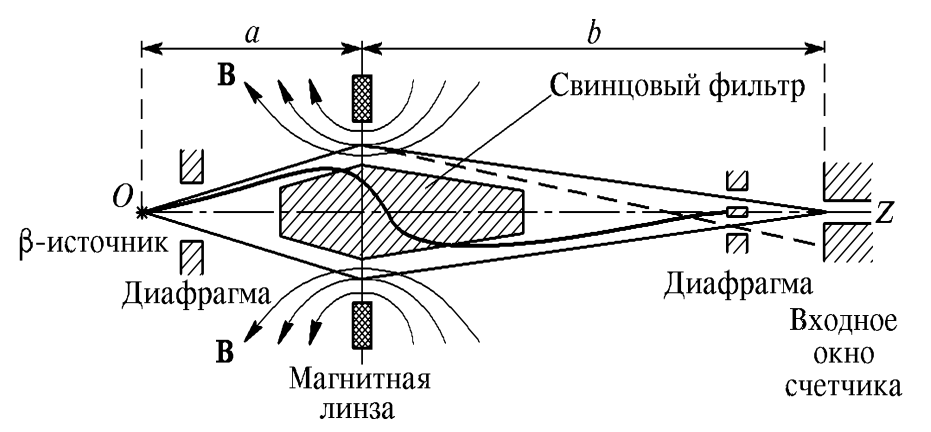
\includegraphics[scale=0.5]{setup.png}
\caption{Схема $\beta$-спектрометра с короткой магнитной линзой}
\end{figure} 

Сама установка состоит из:
\begin{enumerate}
\itemsep0em
\item откаченной трубы, куда помещается радиоактивный источник $^{137}Cs$ 
\item магнитной линзы
\item счетчика
\item компьютера
\item форвакуумного насоса и вакууметра 
\end{enumerate}
\begin{figure}[h!]
\centering
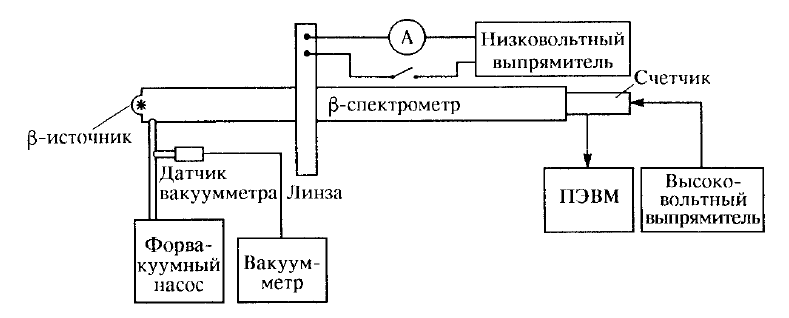
\includegraphics[scale=0.7]{setup (1).png}
\caption{Схема установки для изучения $\beta$-спектра}
\end{figure} 
\paragraph{Ход работы:}
\begin{enumerate}
\itemsep0em
\item В ходе эксперимента были получены данные: 
\begin{figure}[h!]
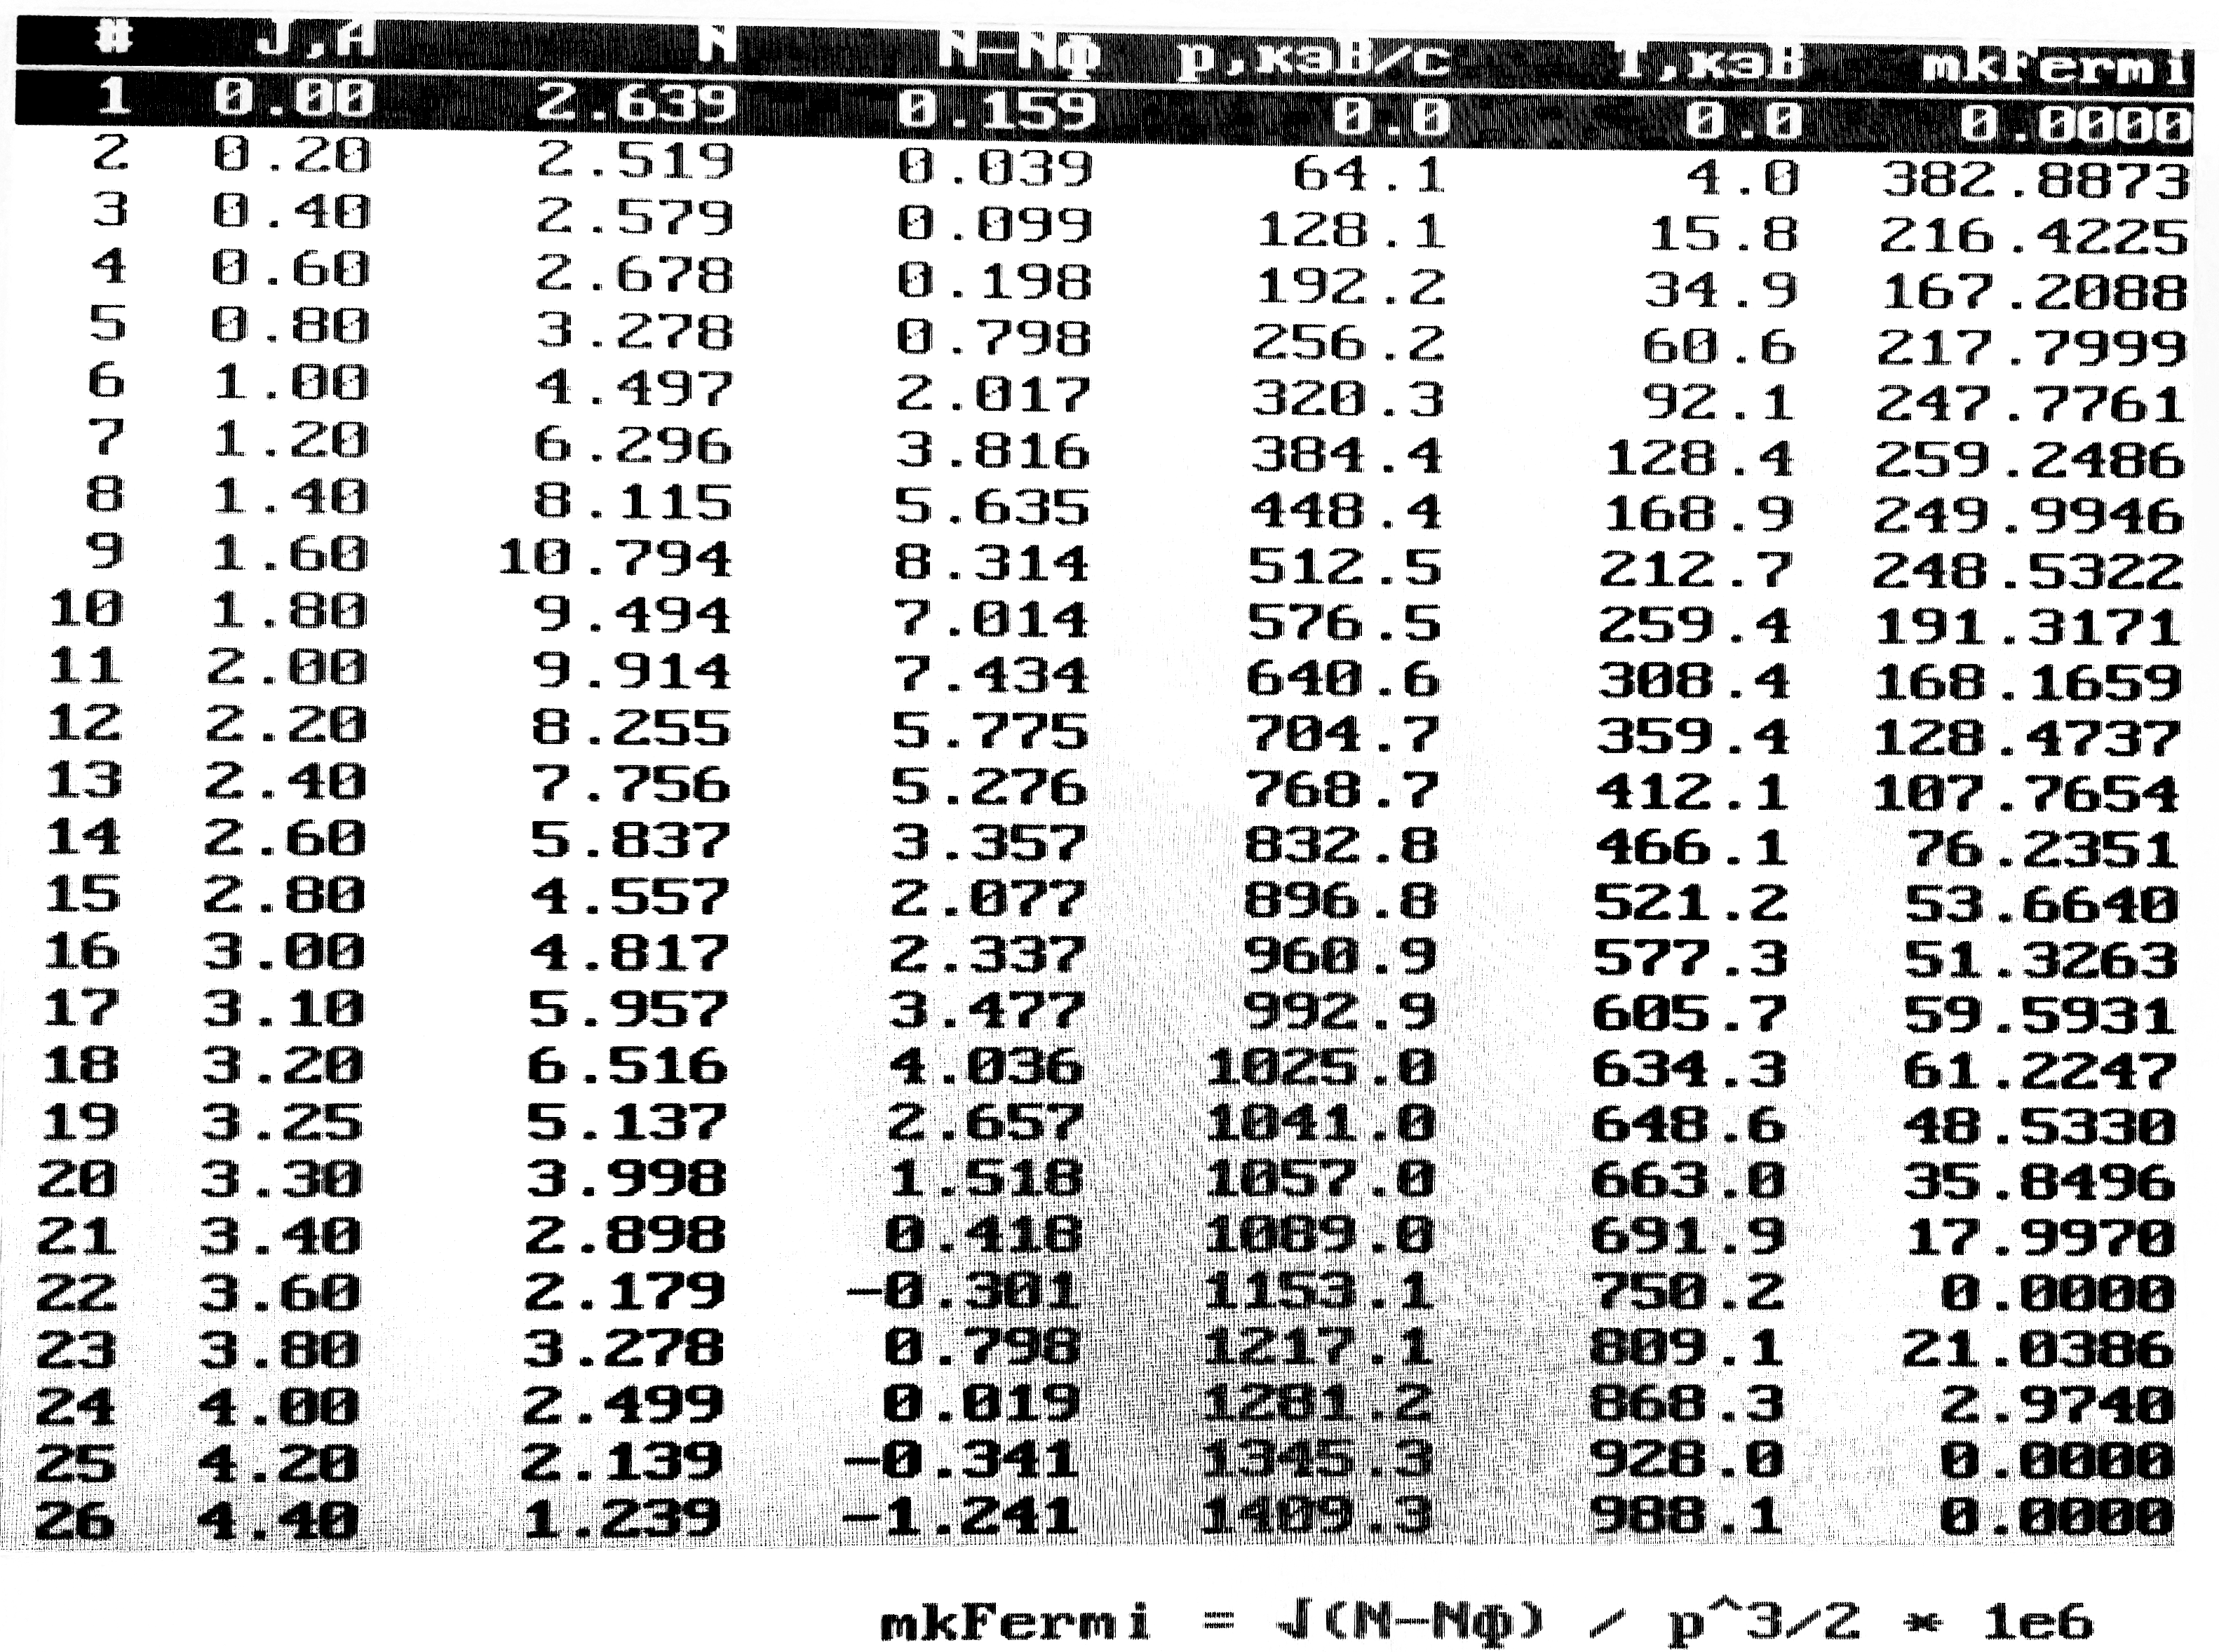
\includegraphics[scale=0.16]{data.png}
\caption{Данные эксперимента} 
\end{figure}
\item Из графика N(p) мы видим ярко выраженный конверсионный пик, произведение импульса на скорость света которого составляет $pc = 1013.5$ кэВ/с. По нему была произведена калибровка спектра.
\begin{figure}[h!]
\centering
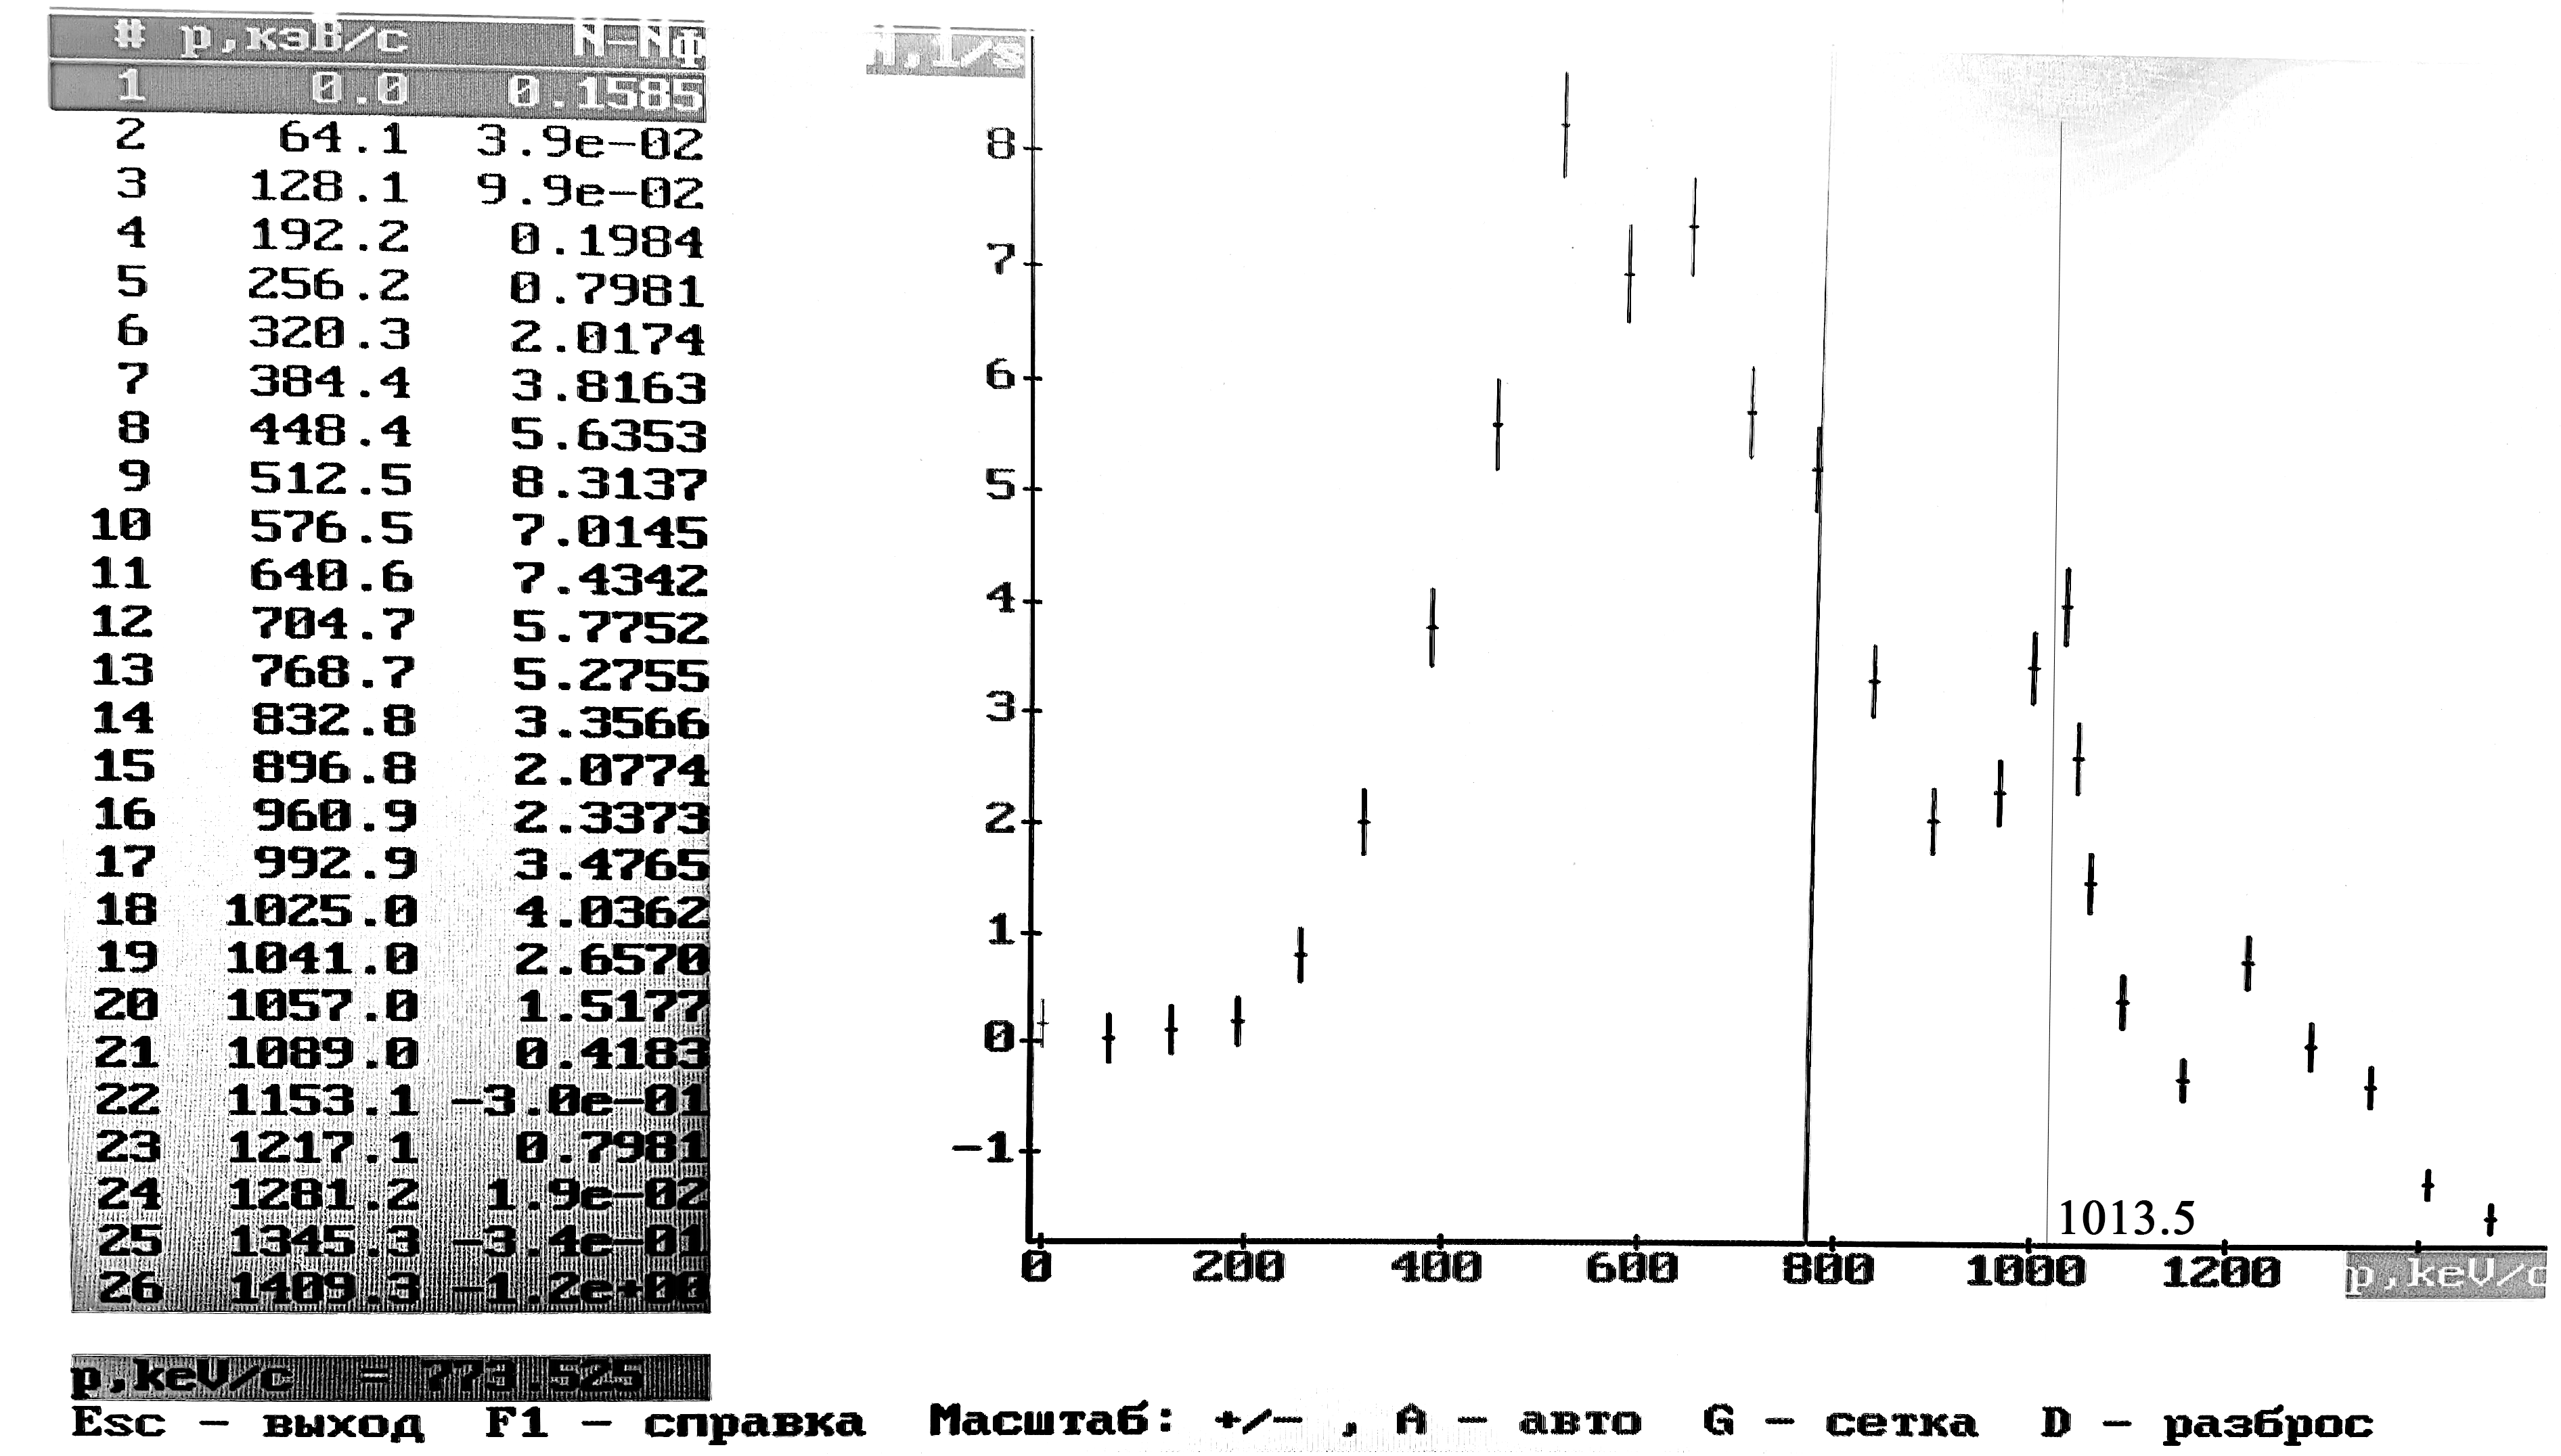
\includegraphics[scale=0.13]{pik.png} 
\end{figure}
\item Получим график Ферми-Кюри. Из него, проведя прямую по МНК получим максимальную энергию $E=E_{max}$ (как прямая, пересекающая ось абсцисс)
\begin{figure}[h!]
\centering
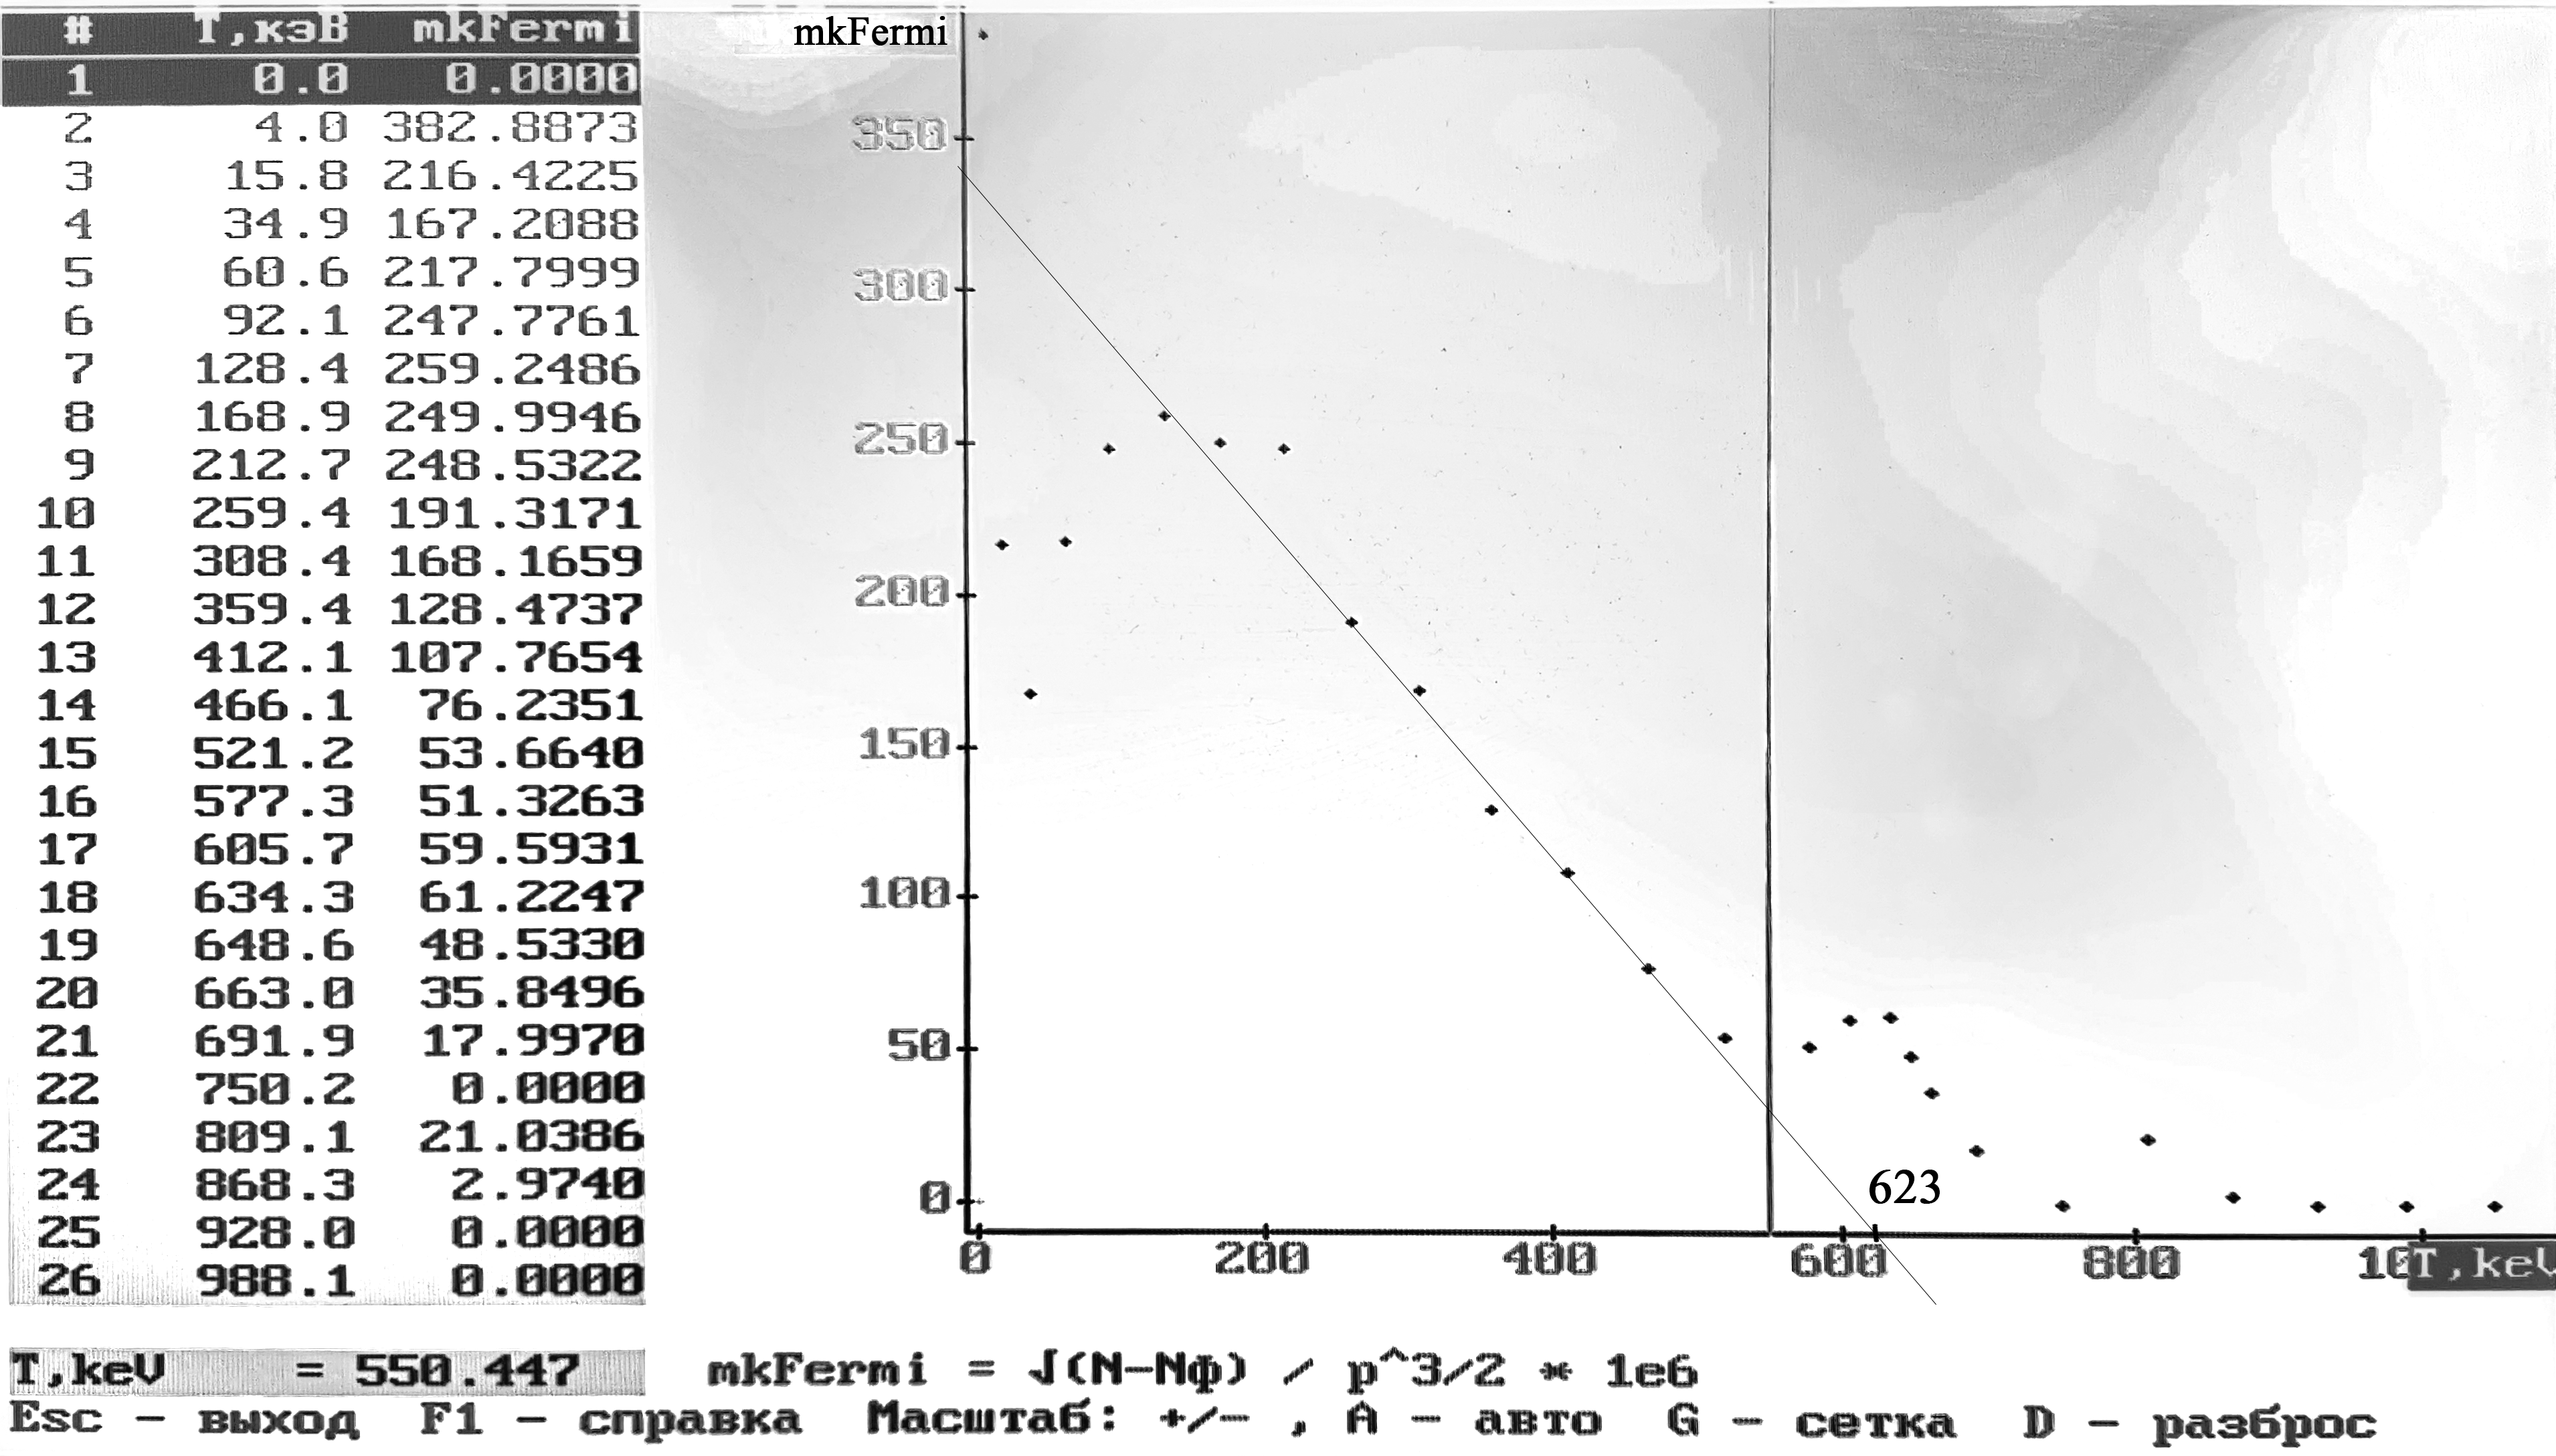
\includegraphics[scale=0.13]{mkFermi.png} 
\end{figure}
\item Из графика, $E_{max}=623$ кэВ
\end{enumerate}
\paragraph{Выводы:}
\begin{enumerate}
\item В ходе работы было исследовано явление $\beta$-распада $^{137}$Cs. В спектре $\beta$-частиц наблюдаются две области: электроны, рождённые в паре с антинейтрино и конверсионные электроны, испускаемые в результате перехода ядра на более низкий энергетический уровень 
\item С помощью графика Ферми-Кюри было определено максимальное значение энергии $\beta$-частиц в спектре: $E_{max} = $ 623 кэВ

\end{enumerate}
\end{document}